% Created 2023-11-13 Mon 19:53
% Intended LaTeX compiler: pdflatex
\documentclass[12pt]{article}
\usepackage[utf8]{inputenc}
\usepackage[T1]{fontenc}
\usepackage{graphicx}
\usepackage{longtable}
\usepackage{wrapfig}
\usepackage{rotating}
\usepackage[normalem]{ulem}
\usepackage{amsmath}
\usepackage{amssymb}
\usepackage{capt-of}
\usepackage{hyperref}
\usepackage[utf8]{inputenc}
\usepackage{sbc-template}
\usepackage{graphicx,url}
\address{Universidade do Sul de Santa Catarina (UNISUL)\\ Tubarão - SC - Brasil\\ anajuliabit@gmail.com}
\usepackage[portuguese, brazilian]{babel}
\usepackage{biblatex}

\addbibresource{references.bib}
\author{Ana Julia Bittencourt Fogaça}
\date{\today}
\title{Análise de Bugs em Contratos Inteligentes de Blockchains Compatíveis com Ethereum Virtual Machine: Janeiro a Setembro de 2023}
\hypersetup{
 pdfauthor={Ana Julia Bittencourt Fogaça},
 pdftitle={Análise de Bugs em Contratos Inteligentes de Blockchains Compatíveis com Ethereum Virtual Machine: Janeiro a Setembro de 2023},
 pdfkeywords={},
 pdfsubject={},
 pdfcreator={Emacs 29.1 (Org mode 9.7)}, 
 pdflang={Portuges}}
\begin{document}

\maketitle

\section{Abstract}
\label{abstract}
Software is developed by humans and, therefore, is inherently subject to flaws and bugs. In the domain of decentralized applications (dApps) operating on the Ethereum Virtual Machine (EVM), these vulnerabilities take on a critical dimension. Unlike conventional software, dApps represent attractive targets for hackers, due to the transparent and open-source nature of blockchains. This article provides a comprehensive analysis of 145 bugs identified in public audits of various projects developed in Solidity and hosted on Ethereum or on EVM-compatible blockchains. Through this analysis, we seek to provide valuable insights into the nature and frequency of vulnerabilities in smart contracts, highlighting the importance of robust development and auditing practices in the blockchain ecosystem.
\section{Resumo}
\label{resumo}
Os softwares são desenvolvidos por humanos e, por isso, estão inerentemente sujeitos a falhas e bugs. No domínio das aplicações descentralizadas (dApps) que funcionam na Ethereum Virtual Machine (EVM), essas vulnerabilidades adquirem uma dimensão crítica. Diferentemente dos softwares convencionais, as dApps representam alvos atraentes para hackers, devido à natureza transparente e de código aberto das blockchains. Este artigo oferece uma análise abrangente de 145 bugs identificados em auditorias públicas de vários projetos desenvolvidos em Solidity e hospedados na Ethereum ou em blockchains compatíveis com EVM. Através desta análise, buscamos fornecer insights valiosos sobre a natureza e a frequência de vulnerabilidades em contratos inteligentes, destacando a importância de práticas de desenvolvimento e auditoria robustas no ecossistema blockchain.
\section{Introdução}
\label{sec:org568cdc3}
Introduzida em 2008 pelo whitepaper do Bitcoin \autocite{nakamotoBitcoinPeertoPeerElectronic}, a tecnologia blockchain é reconhecida como um vetor de transformação em diversas indústrias \autocite{TechnologyTippingPoints}. Caracterizada por sua segurança robusta, transparência e rastreabilidade, além da natureza de código aberto, a blockchain tem encontrado aplicação em operações críticas de negócios. Até 2023, seu uso mais notável, o mercado de criptomoedas, alcançou um valor de mercado superior a um trilhão de dólares \autocite{CryptocurrencyStatistics20232023}. A aplicabilidade da blockchain estende-se além das criptomoedas, impactando setores como finanças, gerenciamento de cadeia de suprimentos, identidade, saúde e governança eleitoral \autocite{BlockchainAdoptionsMaritime}.

A inovação trazida pelo Ethereum, lançado com seu whitepaper em 2014, marcou um ponto de virada na evolução da blockchain. Diferentemente do Bitcoin, que foi concebido primariamente como uma moeda eletrônica peer-to-peer \autocite{nakamotoBitcoinPeertoPeerElectronic}, o Ethereum introduziu o conceito revolucionário de "contratos inteligentes" \autocite{EthereumWhitepaper}. Essa funcionalidade expandiu o escopo de aplicação da blockchain para novas áreas. A plataforma Ethereum destaca-se por sua máquina virtual, capaz de executar códigos em linguagens Turing-complete\autocite{TuringCompleteness2023}. No entanto, como os contratos inteligentes são criados por humanos, eles não estão isentos de falhas. Em um ambiente de código aberto, típico de blockchains como Ethereum, essas falhas podem se tornar alvos atraentes para hackers. Somente no primeiro trimestre de 2023, ataques à rede Ethereum resultaram no roubo de 320 milhões de dólares \autocite{HereHowMuch}. Para mitigar tais riscos, auditorias de contratos inteligentes, sejam privadas, conduzidas por empresas especializadas, ou públicas, através de plataformas como Code4rena \autocite{Code4renaKeepingHigh} e Sherlock \autocite{Sherlock}, são práticas comuns, onde vulnerabilidades podem ser identificadas e os descobridores recompensados.

Desde 2020, projetos de blockchain que negligenciaram o processo de auditoria sofreram perdas financeiras significativas, estimadas em 3.69 bilhões de dólares, enquanto projetos auditados reportaram perdas de 1.3 bilhões \autocite{CompetitiveVsPrivate}. Isso indica que, embora as auditorias reduzam a probabilidade de ataques bem-sucedidos, ainda existem desafios na detecção precoce de vulnerabilidades. Com a demanda crescente por contratos inteligentes e uma projeção de aumento anual de 82,2\% de 2023 a 2030 \autocite{SmartContractsMarket}, torna-se crucial compreender e classificar as vulnerabilidades emergentes. Neste estudo, analisamos 145 bugs identificados em 31 competições de auditoria públicas realizadas entre janeiro e setembro de 2023 nas plataformas renomadas Sherlock \autocite{Sherlock} e Code4rena \autocite{Code4renaKeepingHigh}. Nosso objetivo é elucidar aspectos fundamentais, como a complexidade na detecção de diferentes tipos de bugs e a incidência de categorias específicas de bugs em variados tipos de protocolos.

O artigo está estruturado da seguinte forma: inicialmente, apresentamos uma revisão bibliográfica, abordando os conceitos de blockchain, contratos inteligentes, EVM, Solidity e Finanças descentralizadas. Em seguida, descrevemos a metodologia empregada, a taxonomia e as categorias dos protocolos analisados. Prosseguimos com uma análise dos dados coletados e, por fim, discutimos os resultados obtidos.
\section{Revisão bibliográfica}
\label{sec:orgbfe1d95}
\subsection{Ethereum Blockchain}
\label{sec:org8671608}
A blockchain é um sistema de registro distribuído e imutável que mantém um
registro contínuo da blockchain é um sistema de registro distribuído e imutável
que mantém um registro contínuo de transações ou dados em blocos ligados por
criptografia. Este design assegura a integridade e a veracidade dos dados,
resistindo a alterações retroativas. A Ethereum, conforme delineado no
whitepaper por Vitalik Buterin et al., é uma plataforma blockchain que não só
suporta uma moeda digital, o Ether, mas também permite a construção de
aplicações descentralizadas (dApps) \autocite{EthereumWhitepaper}.
\subsection{Contratos inteligentes}
\label{sec:org4360d91}
Contratos inteligentes são programas que rodam na blockchain do Ethereum,
permitindo que as partes cumpram acordos sem a necessidade de um intermediário.
Uma vez implantados, os contratos inteligentes não podem ser alterados, o que
exige que o código seja verificado para potenciais vulnerabilidades antes do
lançamento. Eles são fundamentais para a finança descentralizada e têm bilhões
de dólares em valor atrelados a eles\autocite{JCPFreeFullText}.
\subsection{Ethereum Virtual Machine}
\label{sec:org93075ac}
A Ethereum Virtual Machine (EVM) é o ambiente de execução para contratos
inteligentes na Ethereum. Funciona como uma camada global que pode executar
código de contrato inteligente em um contexto
descentralizado\autocite{woodETHEREUMSECUREDECENTRALISED}. Isso possibilita que os
desenvolvedores criem aplicações que funcionam exatamente conforme programadas,
sem qualquer possibilidade de fraude ou interferência de terceiros. A EVM é
isolada, significando que o código executado dentro dela não tem acesso ao
sistema de arquivos da rede, a outros contratos inteligentes, ou a qualquer
recurso externo. Esse isolamento garante um alto nível de segurança no
ecossistema Ethereum.
\subsection{Solidity}
\label{sec:org8e8652b}
Solidity é uma linguagem de programação de alto nível para a implementação de
contratos inteligentes e é fortemente tipada, suporta herança, bibliotecas e
tipos de usuário complexos\autocite{SoliditySolidity22}. Projetada para se alinhar
com a EVM, Solidity facilita o desenvolvimento de contratos inteligentes através
de uma sintaxe semelhante a JavaScript, tornando-a acessível a um amplo espectro
de programadores. Solidity, apesar de ser uma linguagem de alto nível com
características robustas, não está isenta de vulnerabilidades. Muitas delas
decorrem de uma desconexão entre a semântica da linguagem e a intuição dos
programadores, principalmente porque Solidity implementa características de
linguagens conhecidas, como JavaScript, de maneiras peculiares. Além disso, a
linguagem carece de construções específicas para lidar com aspectos do domínio
de blockchain, como a imprevisibilidade na ordem ou no atraso das etapas de
computação registradas publicamente na blockchain. Isso ressalta a importância
de uma compreensão aprofundada de Solidity ao desenvolver contratos
inteligentes, para mitigar o risco de vulnerabilidades de segurança.
\subsection{Finanças Descentralizadas}
\label{sec:org3bf65be}
Finanças Descentralizadas (DeFi) representam uma infraestrutura financeira
alternativa construída sobre a tecnologia blockchain, utilizando contratos
inteligentes para replicar serviços financeiros existentes de forma mais aberta,
interoperável e transparente\autocite{scharDecentralizedFinanceBlockchain}​​. DeFi é
uma evolução tecnológica emergente que vem ganhando destaque juntamente com
FinTech, RegTech, criptomoedas e ativos digitais, embora seu significado
completo, implicações legais e consequências políticas ainda sejam pouco
compreendidos​​. Este movimento revolucionário visa criar um sistema financeiro
baseado apenas em código, sem intermediários, e viu um crescimento de ativos
bloqueados de \$4 bilhões para \$104 bilhões em três
anos\autocite{meyerDecentralizedFinanceSystematic2022}​​. Ainda é uma área complexa
que exige uma compreensão rigorosa de suas nuances tanto por praticantes quanto
por pesquisadores de sistemas de
informação\autocite{gramlichMultivocalLiteratureReview2023}​​. Como um novo setor de
tecnologia financeira, DeFi tem o potencial de remodelar a estrutura da finança
moderna e criar um novo cenário para empreendedorismo e inovação, prometendo e
enfrentando desafios e limites​​\autocite{chenBlockchainDisruptionDecentralized2020}.
\section{Metodologia e perguntas da pesquisa}
\label{sec:org83d8556}
\subsection{Categoria dos protocolos}
\label{sec:org40079af}
Os protocolos investigados neste estudo são dedicados ao setor de Finanças
Descentralizadas (DeFi), abarcando exclusivamente as seguintes subcategorias
conforme a classificação proposta por DefiLlama \autocite{DefiLlama}:

\begin{itemize}
\item Derivativos: Protocolos que disponibilizam ferramentas para operações
financeiras alavancadas, possibilitando que os usuários façam previsões e
especulações acerca de valores futuros de ativos, amplificando suas projeções
de lucro ou prejuízo.
\item Yield Farming: Protocolos que incentivam a prática de staking ou fornecimento
de liquidez por parte dos usuários, oferecendo recompensas por tais
atividades.
\item Agregadores de Yield: Protocolos que otimizam os rendimentos por meio da
integração de diversas estratégias de \emph{yield farming}.
\item Opções: Protocolos que ofertam o direito, embora não a obrigação, de adquirir
um ativo por um valor preestabelecido em um momento futuro.
\item DAOs (Organizações Autônomas Descentralizadas): Entidades organizacionais
inovadoras que operam sem centralização, com decisões sendo tomadas de forma
coletiva pelos membros.
\item Launchpads: Protocolos desenvolvidos para lançar novos projetos e criptoativos
no mercado.
\item Índices: Protocolos que rastreiam ou replicam a performance de uma série de
ativos interligados.
\item DEXs (Trocas Descentralizadas): Protocolos que permitem a troca de
criptoativos de forma descentralizada.
\item RWAs (Ativos do Mundo Real): Protocolos relacionados à tokenização de ativos
físicos, como imóveis.
\item Stablecoins: Criptomoedas com valor atrelado a moedas fiduciárias ou outros
ativos, buscando manter sua estabilidade por intermédio de mecanismos
descentralizados.
\item Gestores de Liquidez: Protocolos que gerenciam posições de liquidez em
formadores de mercado automatizados com liquidez concentrada.
\item Empréstimos: Protocolos que permitem o empréstimo e a tomada de empréstimos de
diversos ativos.
\end{itemize}
\subsection{Classificação dos Bugs}
\label{sec:org197d05f}
A classificação das vulnerabilidades dos protocolos analisados neste trabalho
segue uma taxonomia híbrida, combinando os modelos propostos por Zhang et al.
\autocite{zhangDemystifyingExploitableBugs2023a} e as tags de Solodit
\autocite{Solodit_contentReport_tagsMd}, detalhada da seguinte forma:

\begin{itemize}
\item O: Fora do Escopo
\begin{itemize}
\item Inacessibilidade ao código-fonte do projeto.
\item Bugs manifestados em componentes off-chain.
\item Contratos inteligentes desenvolvidos em linguagens distintas
\end{itemize}
\item C01: Manipulação do Mempool / Vulnerabilidades de Front-Running
\begin{itemize}
\item Ataques do tipo sandwich
\item Exploração baseado em \emph{Flash loans}
\end{itemize}
\item C02: Ataque de Reentrada Vulnerabilidades de reentrância, resultantes de
chamadas externas realizadas antes da conclusão de atualizações de estado
internas, possibilitando a um adversário explorar o estado inconsistente.
\item C03: Atualizações de Estado Errôneas. Ausência ou incorreção na atualização de
estado, tal como uma atualização que não deveria ser efetuada.
\item C04: Configuração \emph{Hardcoded} Inserção de valores ou parâmetros estáticos
diretamente no código do contrato inteligente, o que pode representar um risco
de segurança se houver necessidade de flexibilidade.
\item C05: Escalada de Privilégios e Problemas de Controle de Acesso.
\begin{itemize}
\item Chamada de funções privilegiadas sem restrições adequadas.
\item Fundos de usuários que podem ser imobilizados por falhas ou ausência de
código de retirada.
\end{itemize}
\item C06: Matemática Incorreta / Contabilidade Errônea. Erros de cálculo
decorrentes de implementações matemáticas falhas, conduzindo a resultados
imprecisos, incluindo:
\begin{itemize}
\item Ordem incorreta de operações.
\item Retorno de valores inesperados.
\item Utilização de números incorretos para cálculos.
\item Erros de contabilidade.
\item Underflow/overflow.
\end{itemize}
\item C07: Lógica de Negócios Quebrada. Defeitos na lógica de negócios ou protocolos
que, mesmo alinhados à intenção do desenvolvedor, são inerentemente falhos.
\begin{itemize}
\item Invocações de funções inesperadas ou omissas
\item Condições anômalas de ambiente ou contrato
\item Argumentos de função impróprios
\end{itemize}
\item C08: Bugs Específicos da Implementação do Contrato. Bugs que não se enquadram
claramente em outras categorias.
\item C09: Falta de Proteção Contra Replay de Assinatura
\begin{itemize}
\item Nonce ausente
\item Colisão de hash
\end{itemize}
\item C10: Verificação Ausente. Omissão crítica de condições ou validações
essenciais no código.
\item C11: DoS (Negação de Serviço). Vulnerabilidades que permitem a um atacante
comprometer a resposta ou eficiência do contrato. Esta categoria inclui casos
que não são bem descritos por outra classe e onde a consequência primária é o
encerramento do contrato ou ineficiência operacional.
\item C12: Validação de Dados Falhas na verificação ou saneamento de entradas,
particularmente daquelas oriundas de fontes externas.
\item C13: Correspondência de Lista Branca/Lista Negra. Gerenciamento inadequado de
endereços baseado em listas predefinidas.
\item C14: Arrays. Vulnerabilidades associadas ao manuseio inadequado de arrays,
incluindo:
\begin{itemize}
\item Leituras/escritas fora dos limites
\item Problemas na exclusão
\item Questões relacionadas ao redimensionamento de arrays
\end{itemize}
\end{itemize}
\subsection{Coleta de dados}
\label{sec:orge102333}
\begin{table}[htbp]
\caption{\label{TABELA1}Visão Geral das Competições Avaliadas. 'HRF' (High Risk Findings) representa bugs de alta severidade. 'nSLOC' indica o número total de linhas de código associadas a cada competição.}
\centering
\begin{tabular}{lllrrrrr}
Plataforma & Categoria & Competição & Prêmio & HRF & nSLOC & Participantes & Data\\[0pt]
\hline
Code4rena & DAO & \href{https://code4rena.com/reports/2023-08-arbitrum}{Arbitrum security council election} & 90500 & 1 & 2184 & 39 & 2023-09\\[0pt]
Code4rena & DAO & \href{https://code4rena.com/reports/2023-06-llama}{Llama} & 60500 & 2 & 2096 & 50 & 2023-07\\[0pt]
Code4rena & Stablecoin & \href{https://code4rena.com/reports/2023-06-lybra}{Lybra finance} & 60500 & 8 & 1762 & 136 & 2023-08\\[0pt]
Code4rena & Dexes & \href{https://code4rena.com/reports/2023-05-maia}{Maia DAO ecosystem} & 300500 & 35 & 10997 & 85 & 2023-05\\[0pt]
Code4rena & Yield & \href{https://code4rena.com/reports/2023-07-pooltogether\#wardens}{PoolTogether} & 121650 & 9 & 3324 & 117 & 2023-07\\[0pt]
Code4rena & Yield & \href{https://code4rena.com/reports/2023-08-pooltogether}{PoolTogether v5: part deux} & 42000 & 2 & 1001 & 45 & 2023-08\\[0pt]
Sherlock & Lending & \href{https://audits.sherlock.xyz/contests/75}{Ajna update} & 85600 & 6 & 5659 & 155 & 2023-06\\[0pt]
Sherlock & Yield Agreggator & \href{https://audits.sherlock.xyz/contests/41}{Blueberry} & 72500 & 10 &  & 284 & 2023-02\\[0pt]
Sherlock & Yield Agreggator & \href{https://audits.sherlock.xyz/contests/104/report}{Blueberry Update \#3} & 23600 & 5 & 3633 & 183 & 2023-08\\[0pt]
Sherlock & Opções & \href{https://audits.sherlock.xyz/contests/99}{Bond options} & 23600 & 2 & 885 & 153 & 2023-07\\[0pt]
Sherlock & Empréstimos & \href{https://audits.sherlock.xyz/contests/107}{Cooler update} & 17000 & 4 & 512 & 170 & 2023-08\\[0pt]
Sherlock & Dexes & \href{https://audits.sherlock.xyz/contests/97}{GFX labs} & 20400 & 2 & 716 & 106 & 2023-07\\[0pt]
Sherlock & Derivativos & \href{https://audits.sherlock.xyz/contests/74}{GMX} & 200000 & 5 & 10571 & 220 & 2023-04\\[0pt]
Sherlock & Lending & \href{https://audits.sherlock.xyz/contests/84}{Iron bank} & 67400 & 1 & 2241 & 271 & 2023-05\\[0pt]
Sherlock & Derivativos & \href{https://audits.sherlock.xyz/contests/79}{Perennial} & 122000 & 1 & 4063 & 220 & 2023-05\\[0pt]
Sherlock & Derivativos & \href{https://audits.sherlock.xyz/contests/106}{Perennial v2} & 125200 & 6 & 2494 & 252 & 2023-07\\[0pt]
Sherlock & Derivativos & \href{https://audits.sherlock.xyz/contests/85}{Symmetrical} & 91000 & 8 & 3553 & 233 & 2023-06\\[0pt]
Sherlock & Derivativos & \href{https://audits.sherlock.xyz/contests/108}{Symmetrical Update} & 27600 & 2 & 3921 & 52 & 2023-08\\[0pt]
Sherlock & Launchpad & \href{https://audits.sherlock.xyz/contests/100}{Tokensoft} & 21400 & 1 & 769 & 221 & 2023-07\\[0pt]
Sherlock & Stablecoin & \href{https://audits.sherlock.xyz/contests/73}{Unitas protocol} & 36400 & 1 & 1433 & 208 & 2023-06\\[0pt]
Code4rena & RWA & \href{https://code4rena.com/contests/2023-01-ondo-finance-contest}{Ondo finance} & 60500 & 1 & 4365 & 74 & 2023-01\\[0pt]
Sherlock & Índices & \href{https://audits.sherlock.xyz/contests/81}{Index coop} & 130600 & 2 & 4383 & 283 & 2023-05\\[0pt]
Sherlock & Stablecoin & \href{https://audits.sherlock.xyz/contests/82}{USSD} & 18200 & 3 & 402 & 224 & 2023-05\\[0pt]
Sherlock & RWA & \href{https://audits.sherlock.xyz/contests/98}{Dinari} & 16000 & 1 & 575 & 176 & 2023-07\\[0pt]
Sherlock & Dexes & \href{https://audits.sherlock.xyz/contests/88}{RealWagmi} & 33200 & 5 & 1080 & 203 & 2023-06\\[0pt]
Code4rena & DAO & \href{https://code4rena.com/reports/2023-07-nounsdao}{Nouns DAO} & 100000 & 1 & 9098 & 36 & 2023-07\\[0pt]
Sherlock & Dexes & \href{https://audits.sherlock.xyz/contests/89}{DODO v3} & 57800 & 5 & 2079 & 151 & 2023-06\\[0pt]
Sherlock & Derivativos & \href{https://audits.sherlock.xyz/contests/72}{Hubble Exchange} & 60000 & 3 & 1945 & 148 & 2023-06\\[0pt]
Code4rena & Stablecoin & \href{https://code4rena.com/contests/2023-06-angle-protocol-invitational}{Angle Protocol} & 52500 & 3 & 2276 & 5 & 2023-07\\[0pt]
Code4rena & Gestores de liquidez & \href{https://audits.sherlock.xyz/contests/86}{Arrakis} & 81400 & 2 & 2801 & 247 & 2023-06\\[0pt]
Sherlock & Dexes & \href{https://audits.sherlock.xyz/contests/95}{Unstoppable} & 36400 & 8 & 2035 & 130 & 2023-06\\[0pt]
\hline
TOTALS &  &  & 2255950 & 145 & 3095.1 & 157.32258 & \\[0pt]
\end{tabular}
\end{table}

No período de janeiro a setembro de 2023, nossa análise focou em 31 das
competições de auditoria pública realizadas nas plataformas Code4rena
\autocite{Code4renaKeepingHigh} e Sherlock \autocite{timeMostInterestingWeb32023}, nas
quais foram identificados 145 bugs de alta severidade. Com duração média de sete
dias, estes eventos visaram a identificação de falhas críticas em contratos
inteligentes antes de seu lançamento final. A \hyperref[TABELA1]{Tabela 1} detalha as competições
examinadas, incluindo o número de participantes, o prêmio total, a categoria do
projeto, a quantidade de vulnerabilidades de alta severidade encontradas e o
total de linhas de código abrangidas em cada competição. O valor total das
recompensas distribuídas nesses eventos superou os dois milhões de dólares, com
uma média de 150 participantes por evento. Após a fase de submissão, juízes
especializados em auditoria de contratos inteligentes, selecionados pela
comunidade, avaliaram a severidade dos bugs. Os bugs classificados como de alta
severidade representam riscos significativos, incluindo a possibilidade de roubo
ou perda de ativos digitais \autocite{JudgingCriteria}. Todos os bugs, suas
descrições e a classificação realizada estão disponíveis no nosso dataset
\autocite{bittencourtSolidityCommonVulnerabilities2023}
\section{Análise e Discussão dos Resultados}
\label{sec:orgf0a3d46}
\begin{figure}[h]
  \centering
  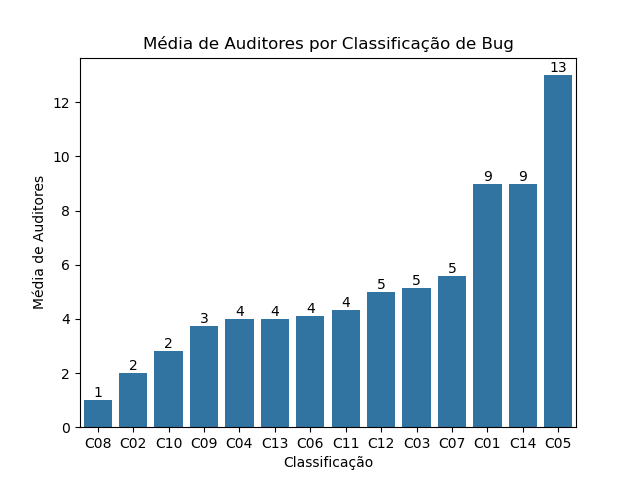
\includegraphics[width=\linewidth]{../results/average_auditors_by_class.png}
  \caption{Média de auditores por classificação}

  \label{fig:grafico_1}
\end{figure}

\begin{figure}[h]
  \centering
  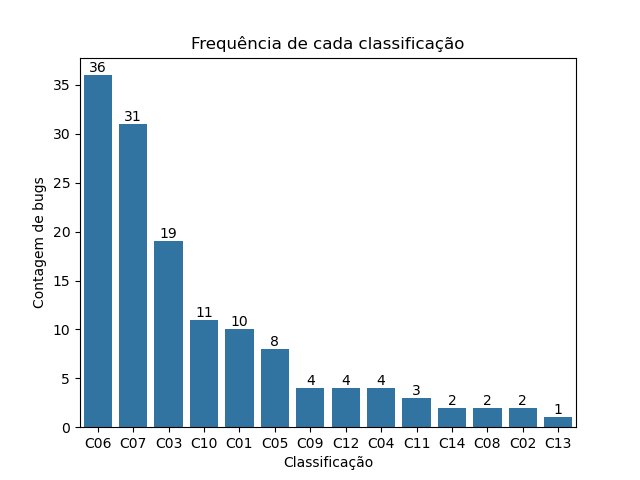
\includegraphics[width=\linewidth]{../results/bugs_by_class.png}
  \caption{Contagem de Bugs por Classificação}

  \label{fig:grafico_2}
\end{figure}

\begin{figure}[h]
  \centering
  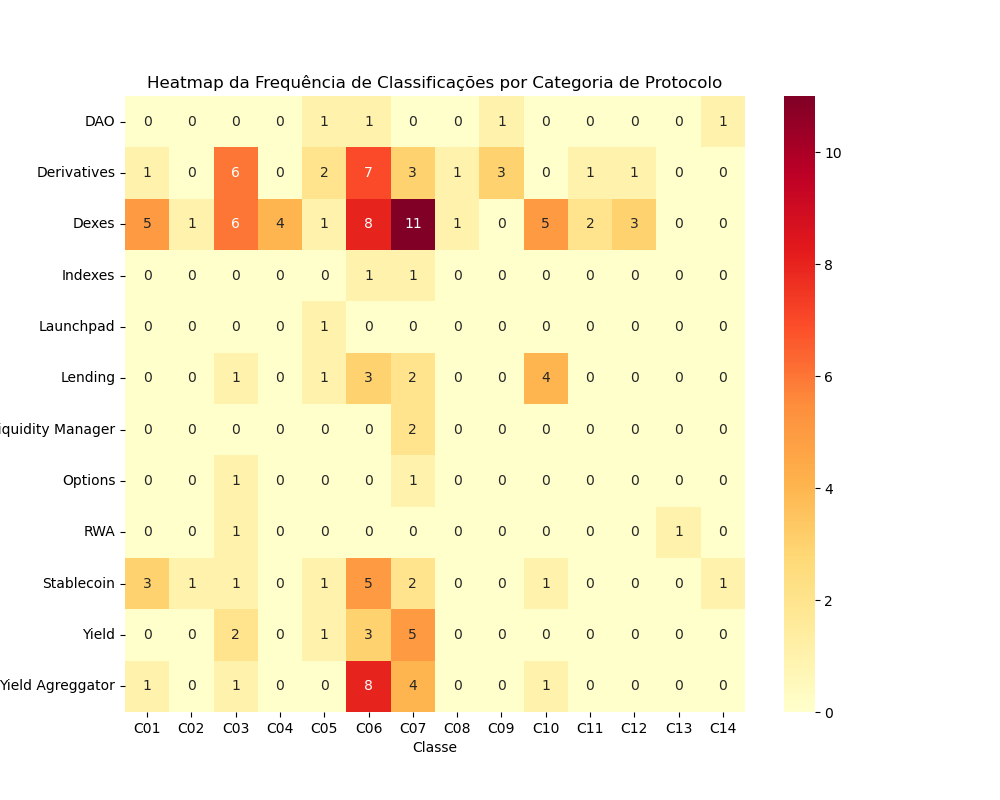
\includegraphics[width=\linewidth]{../results/bugs_by_protocol_category_with_class_as_hue.png}
  \caption{Frequência de Classificações por Categoria de Protocolo}

  \label{fig:grafico_3}
\end{figure}

\begin{figure}[h]
  \centering
  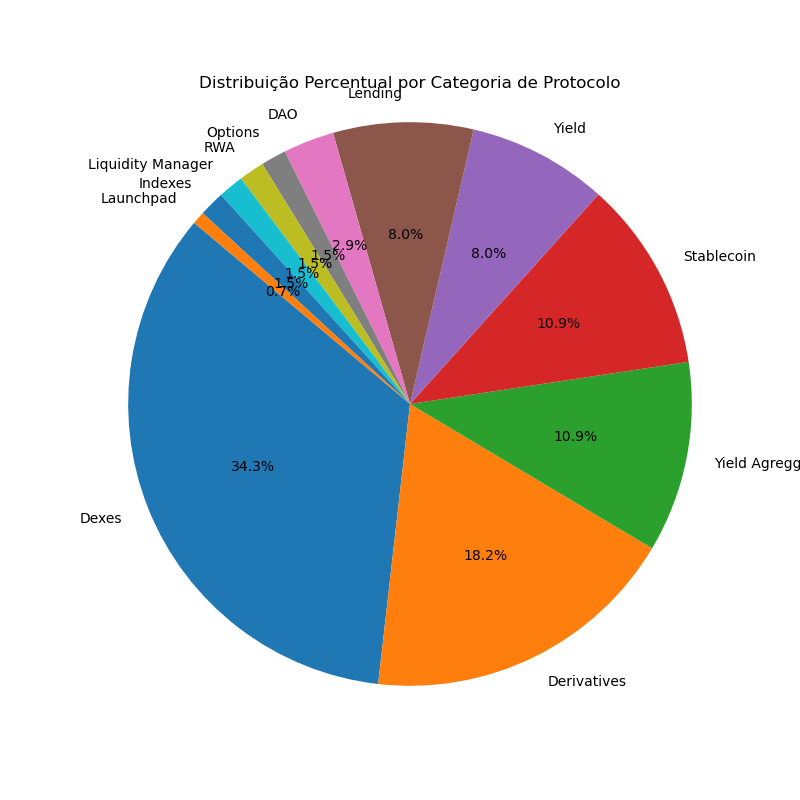
\includegraphics[width=\linewidth]{../results/bugs_by_protocol_category.png}
  \caption{Distriuição Percentual por Categoria de Protocolo}

  \label{fig:grafico_3}
\end{figure}
\subsection{Análise dos dados coletados}
\label{sec:org6bb00d9}
A identificação de vulnerabilidades em contratos inteligentes é uma tarefa que
exige extrema atenção aos detalhes e uma mentalidade orientada para a descoberta
de falhas, similar à de um potencial atacante. Neste contexto, auditores
enfrentam desafios significativos na condução de suas investigações,
especialmente porque muitos bugs permanecem não detectados
\autocite{CompetitiveVsPrivate}. Para aprofundar nosso entendimento desses
desafios, conduzimos uma análise exploratória do dataset, utilizando as
bibliotecas Python Panda e Seaborn. O script utilizado nessa análise está
documentado em \autocite{bittencourtSolidityCommonVulnerabilities2023}, e todos os
gráficos nesta seção foram gerados a partir dele.

Nossas principais descobertas incluem:

\begin{enumerate}
\item A detecção de bugs por um número reduzido de auditores sugere uma
complexidade elevada em sua identificação. Como ilustrado na Figura 1, entre
as diversas categorias de vulnerabilidades, aquelas relacionadas a Falhas
Específicas na Implementação de Contratos (C08), seguidas por
Vulnerabilidades de Reentrância (C02) e Ausência de Verificações (C10),
emergem como as mais desafiadoras. Em contraste, categorias como Problemas de
Controle de Acesso e Escalada de Privilégios (C05), Arrays (C14), e
Manipulação de Mempool / Vulnerabilidades de Front-Running (C01) são mais
facilmente identificáveis.

\item C06 - Erros de Cálculo (Matemática Incorreta/Contabilidade Errônea): Conforme
a Figura 2, essa categoria é a mais prevalente, indicando que falhas em
lógica matemática, como underflows/overflows ou sequências erradas de
operações, são comuns no setor de Finanças Descentralizadas (DeFi). Isso é
compreensível, considerando a complexidade dos cálculos matemáticos no DeFi.
Essa observação sugere que muitos contratos inteligentes são vulneráveis
devido a implementações inadequadas de operações matemáticas, resultando
potencialmente em perdas financeiras significativas.

\item C07 - Lógica de Negócios Quebrada: Esta é a segunda classificação mais comum,
como mostra a Figura 2, indicando que muitos contratos têm falhas na lógica
de negócios, que poderiam ser mitigadas com análises e testes mais detalhados
das regras de negócio e cenários de contrato.

\item C03 - Atualizações de Estado Errôneas: Esta classificação, a terceira em
frequência, sugere que uma parcela significativa de contratos possui falhas
na lógica que gerencia o estado do contrato, levando a consequências
imprevistas e possíveis vulnerabilidades de segurança.

\item Classes Menos Frequentes (C02, C08, C13): Vulnerabilidades como Reentrância
(C02) e Falhas Específicas na Implementação de Contratos (C08) são menos
frequentes, conforme a Figura 2, o que pode indicar maior dificuldade de
detecção, alinhando-se com a descoberta 1 de que C02 e C08 são categorias
desafiadoras. A classe C13, que inclui vulnerabilidades como o uso de funções
de hash inseguras, também é menos frequente.

\item Classes dominantes de vulnerabilidades, como Lógica de Negócios Quebrada
(C07), Atualizações de Estado Incorretas (C03), Problemas de Controle de
Acesso e Escalada de Privilégios (C05), e Erros de Cálculo (C06), são
recorrentes em várias categorias, conforme indica a Figura 3. Esses padrões
reforçam a prevalência destes tipos de vulnerabilidades.

\item Diferentes categorias de protocolo apresentam distintos perfis de
vulnerabilidade. Protocolos Dexes registraram o maior número de bugs, com
34.3\% dos bugs identificados pertencendo a esta categoria, seguido por
Derivativos com 18.2\%, e Agregadores e Stablecoins com aproximadamente 10\%
cada, conforme ilustrado na Figura 4.
\end{enumerate}
\subsection{Discussão dos Resultados}
\label{sec:org0fb19b8}
Esta seção visa aprofundar a análise dos resultados obtidos e explorar suas
implicações práticas

\begin{enumerate}
\item Complexidade na Identificação de Vulnerabilidades: Os resultados revelam uma
complexidade considerável na detecção de certas categorias de
vulnerabilidades, especialmente aquelas relacionadas a falhas específicas na
implementação de contratos e vulnerabilidades de reentrância. Isso enfatiza a
necessidade de ferramentas e métodos de auditoria mais sofisticados, assim
como a importância de uma formação contínua para desenvolvedores e auditores,
a fim de equipá-los com as habilidades necessárias para identificar tais
vulnerabilidades.

\item Foco na Verificação de Lógica Matemática: A prevalência de erros de cálculo
no DeFi sugere a necessidade de uma maior atenção na verificação de lógicas
matemáticas e operações contábeis. Práticas como testes de fuzzing, revisões
de código por pares e simulações podem ser essenciais para prevenir falhas.

\item Vulnerabilidades na Lógica de Negócios e Atualizações de Estado: A frequência
dessas categorias de vulnerabilidades aponta para a necessidade de uma
análise mais profunda da lógica de negócios e dos mecanismos de atualização
de estado nos contratos inteligentes. Este aspecto sublinha a importância de
um design de contrato cuidadoso, além de testes abrangentes e análises de
cenários para garantir a integridade do contrato.

\item Diferentes Perfis de Vulnerabilidade em Diferentes Protocolos: A análise
destacou variações significativas nos perfis de vulnerabilidade entre
diferentes tipos de protocolos de blockchain, como Dexes, Derivativos e
Stablecoins. Isso implica que estratégias de segurança e auditoria devem ser
adaptadas conforme o tipo de protocolo, considerando suas características e
riscos específicos.
\end{enumerate}
\section{Considerações finais}
\label{sec:org453b299}
Este estudo analisa 145 bugs identificados em competições de auditorias públicas, destacando aspectos cruciais e desafios relacionados à segurança de contratos inteligentes. As descobertas principais indicam a complexidade na identificação de vulnerabilidades específicas, sublinhando a necessidade de ferramentas e habilidades de auditoria avançadas. Notavelmente, a prevalência de erros de cálculo no setor de Finanças Descentralizadas (DeFi) e falhas na lógica de negócios ressalta a importância de verificar rigorosamente as operações matemáticas e analisar detalhadamente a lógica de negócios. Os resultados enfatizam a necessidade de uma abordagem holística e meticulosa no desenvolvimento e na auditoria de contratos inteligentes, destacando a importância de ferramentas de análise mais sofisticadas, educação contínua para desenvolvedores e auditores, e a adoção de práticas rigorosas de teste e validação. Para futuras pesquisas, recomenda-se a exploração de métodos de inteligência artificial e aprendizado de máquina na detecção e análise de vulnerabilidades. Estas tecnologias podem oferecer uma análise mais aprofundada e abrangente, identificando padrões complexos e sutilezas. Além disso, a colaboração entre comunidades acadêmicas, desenvolvedores de blockchain e profissionais de segurança cibernética é sugerida para estabelecer benchmarks e frameworks padronizados para a avaliação de segurança em contratos inteligentes. Essa colaboração pode levar ao desenvolvimento de melhores práticas, diretrizes de codificação segura e ferramentas de auditoria mais robustas, contribuindo significativamente para a segurança no ecossistema de Finanças Descentralizadas (DeFi).

\printbibliography
\end{document}